\documentclass{article}

% \usepackage{nips_2018} % ready for submission
% \usepackage[preprint]{nips_2018} % compile a preprint version
% \usepackage[final]{nips_2018} % to compile a camera-ready version
% \usepackage[nonatbib]{nips_2018} % to avoid loading the natbib package
\usepackage[preprint, nonatbib]{nips_2018}

\usepackage{graphicx}
\graphicspath{ {./images/} }
\usepackage{subfig}
\usepackage{color,soul}
\usepackage{amsmath}
\usepackage{amssymb}
\usepackage[utf8]{inputenc} % allow utf-8 input
\usepackage[T1]{fontenc}    % use 8-bit T1 fonts
\usepackage{hyperref}       % hyperlinks
\usepackage{url}            % simple URL typesetting
\usepackage{booktabs}       % professional-quality tables
\usepackage{amsfonts}       % blackboard math symbols
\usepackage{microtype}      % micro-typography
\usepackage{cite}
\usepackage{color}
\usepackage{algorithmicx}
\title{Proactive Caching with Deep Reinforcement Learning}

\author{
  HONG Yuncong \\
  Department of Computer Science \\
  The University of Hong Kong \\
  \texttt{ychong@cs.hku.hk} \\
  \And % Using \AND forces a line break at that point
  ZENG Qunsong \\
  Department of Electrical and Electronic Engineering \\
  The University of Hong Kong \\
  \texttt{qszeng@eee.hku.hk} \\
}

\begin{document}

\maketitle

\begin{abstract}
  In next-generation networks, proactive edge caching is a promising technique to reduce the data traffic while improve the quality of experience of users. However, it is challenging to solve the edge caching problem with unknown future content popularity and complex network characteristics. Inspired by the success of \emph{Deep Reinforcement Learning} (DRL) in solving complicated decision making problem, this work presents a DRL-based framework for proactive edge caching. Our goal is to minimize the expected long-term average re-buffering download time. To evaluate the proposed framework, we compare the performance with \emph{Least Recently Used} (LRU) caching strategy. Our results show that the proposed DRL-based algorithm can achieve better performance in comparison with LRU scheme.
\end{abstract}

\begin{section}{Introduction}
    \label{sec:intro}
    Content caching is a promising technology in system to reduce the load on access communication links and shorten access time to the selected contents \cite{general-cache}. This technique is aimed at pre-caching the contents at the edge from the cloud server in advance. In this particular way, the time and resources needed to request and transport contents from upper level cloud server can be effectively saved.
    
    % As for caching placement problem, one practical design is content delivery network (CDN) which is a network of servers linked together in order to deliver contents with high performance \cite{cloudflare}. Emerging areas, such as information centric networks (ICNs) and cloud computing frameworks, \cite{ref1,ref2,ref3,ref4} are based on caching problem and are attracting researchers' attention. Many algorithms for caching placement problems are elaborated in related works \cite{dl-mec,dl-icn,expert-cdn}.
    
    However, for proactive edge caching, we have to explore and decide which files or contents to store in caches, which leads to the policy control problem \cite{DBLP:journals/corr/abs-1712-08132}. Although many related works have exploited their algorithms, few of them can adapt to the online production environment with complicated control problem very well. Inspired by \emph{Deep Reinforcement Learning} (DRL) method, we propose a DRL-based framework "AutoCache" for caching decisions. In this paper, we design a DRL agent for segment caching decisions at an edge node. Users keep requesting file from the edge node, which is supposed as a queue of requests to be served. The edge cache has a fixed storage capacity, which is the maximum file segments that can be cached at this node. Furthermore, we present the simulation results to validate the effectiveness of the proposed AutoCache algorithm for edge caching.
    
    To the best known of authors' knowledge, this work makes the first attempt to consider the two-phase request model with deep reinforcement learning framework for edge caching. We propose a novel algorithm "AutoCache" to solve policy control issues in align with our model implementation. The simulation results are compared with the classical LRU caching policy to clarify the performance of our new method. The comparison shows the proposed DRL-based algorithm outperforms the LRU caching policy for edge caching.
\end{section}

\begin{section}{Related Works}
    \label{sec:review}
    Proactive content caching is an active area in networks, which has attracted much attention of researchers. From the aspect of big data, the proactive caching is discussed with regard to the improvement of user experience and reduction of data traffic \cite{rw1}. The study in \cite{rw3} proposed an age-based threshold policy which caches all contents that have been requested more than a threshold. In addition, some popularity-based content caching policies, such as StreamCache in \cite{rw4} and PopCaching in \cite{rw5}, are studied. Recently, researchers are paying more attention to machine learning based methods. In \cite{rw2}, the authors studied three learning based content replacement algorithms with different exploration-exploitation trade-offs. In the context of uncertain content popularity, the multi-armed bandit learning algorithm is used for estimation of content popularity in \cite{rw6} and an extreme-learning machine framework is proposed for content popularity prediction in \cite{rw7}.
    
    As illustrated in previous related works, the key to solve the content caching problem is the content popularity distribution estimation. Considering the complex network environment and the uncertain popularity, some researchers introduce deep reinforcement learning as the strategy to solve the problem. For example, the multi-step return actor-critic architecture, a typical DRL algorithm, is proposed to apply in proactive caching \cite{rw8}. In \cite{Pensieve}, a system named Pensieve that generates \emph{adaptive bitrate} (ABR) algorithms using DRL is proposed for video chunks caching. More recently, the application of DRL in mobile edge caching is discussed in details \cite{MEC}. The simulation results in these works show good performance of DRL algorithms with policy problem, which motivates more researchers to implement more DRL-based model for various scenarios.
\end{section}

\begin{section}{Background}
    \label{sec:background}
    \subsection{Edge Caching}
    Nowadays, the number of files available over the Internet is extremely huge. Considering the storage space of edge nodes is limited, there exists a policy problem to decide how to store the files in the cache. For this problem, the popularity of content should be taken into consideration. Usually, it is assumed that content popularity follows a static Zipf distribution \cite{7524380}. However, since the the user preferences may be changing and uncertain with time, the true distribution of content popularity is unknown and complex \cite{7524790}.
    
    The objective of caching policies is commonly related to the cache hit ratio, which is the probability that the contents requested by users are cached in the edge networks. Some conventional caching policies, such as LRU and LFU, have been widely used in caching systems, but these policies perform not well in edge caching, especially mobile edge caching systems, due to being unable to consider the changes and uncertainty in the operating environments.
    
    \begin{figure}[h!]
        \centering
        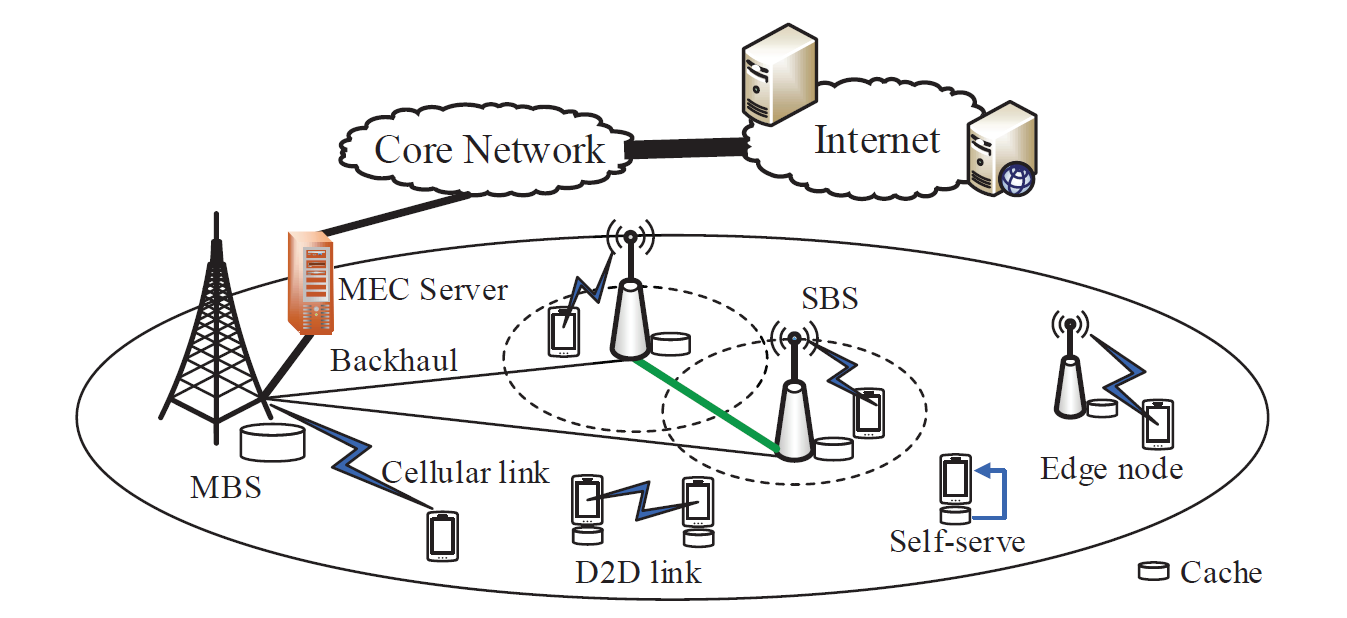
\includegraphics[width=0.8\linewidth]{images/cache.png}
        \caption{Architecture of edge caching \cite{MEC}}
        \label{fig:network}
    \end{figure}
    
    \subsection{Deep Reinforcement Learning}
    The standard reinforcement learning setting is where an agent interacts with an environment over a number of discrete time steps \cite{DBLP:journals/corr/MnihBMGLHSK16}. At each time step $t$, the agent receives a state $s_t$ and selects an action $a_t$ from some set of possible action $\mathcal{A}$ according to its policy $\pi$, where $\pi$ is a mapping from states $s_t$ to actions $a_t$. In return, the agent receives the next state $s_{t+1}$ and receives a reward $r_t$. The process continues until the agent reaches a terminal state after which the process restarts. The return $R_t=\sum_{k=0}^{\infty}\gamma^kr_{t+k}$ is the total accumulative return from time step $t$ with discount factor $\gamma\in(0,1]$. The goal of the agent is to maximize the expected return from each state $s_t$. The action value $Q^{\pi}(s,a)=\mathbb{E}[R_t|s_t=s,a]$ is the expected return for selecting action $a$ in state $s$ and following policy $\pi$. The optimal value function $Q^*(s,a)=\max_{\pi}Q^{\pi}(s,a)$ gives the maximum action value for state $s$ and action $a$ achievable by any policy. The value of state $s$ under policy $\pi$ is defined as $V^{\pi}(s)=\mathbb{E}[R_t|s_t=s]$ and is simply the expected return for following policy $\pi$ from state $s$ \cite{DBLP:journals/corr/MnihBMGLHSK16}.
    
    Q-learning is a value-based off-policy method. In deep Q-Learning, the deep neural network is used to be a function approximator to estimate the action-value function: $Q(s,a;\theta)\approx Q^*(s,a)$, where the weight parameters of the deep neural network is $\theta$. The loss function can be defined as
    $$
    L_{i}\left(\theta_{i}\right)=\mathbb{E}_{s, a \sim \rho(\cdot)}\left[\left(y_{i}-Q\left(s, a ; \theta_{i}\right)\right)^{2}\right]
    $$
    where
    $$
    y_{i}=\mathbb{E}_{s^{\prime} \sim \mathcal{S}}\left[r+\gamma \max _{a^{\prime}} Q\left(s^{\prime}, a^{\prime} ; \theta_{i-1}\right) | s, a\right]
    $$
    Then the problem can be solved by gradient update
    $$
    \nabla_{\theta_{i}} L_{i}\left(\theta_{i}\right)=\mathbb{E}_{s, a \sim \rho(\cdot)}\left[\left(r+\gamma \max _{a^{\prime}} Q\left(s^{\prime}, a^{\prime} ; \theta_{i-1}\right)-Q\left(s, a ; \theta_{i}\right)\right) \nabla_{\theta_{i}} Q\left(s, a ; \theta_{i}\right)\right]
    $$
    Policy Gradients methods are policy-based, which directly optimize the policy space. For each policy $\pi_{\theta}$, define its value as follows.
    $$
    J(\theta)=\mathbb{E}\left[\sum_{t \geq 0} \gamma^{t} r_{t} | \pi_{\theta}\right]
    $$
    so the optimal policy is given by $\theta^*=\arg\max_{\theta}J(\theta)$.
    When sampling a trajectory $\tau$, we can estimate $J(\theta)$ with
    $$
    \nabla_{\theta} J(\theta) \approx \sum_{t \geq 0} r(\tau) \nabla_{\theta} \log \pi_{\theta}\left(a_{t} | s_{t}\right)
    $$
    We want to push up the probability of an action from a state, if this action was better than the expected value of what we should get from that state. Especially, we favor an action $a_t$ in a state $s_t$ if $Q^{\pi}\left(s_{t}, a_{t}\right)-V^{\pi}\left(s_{t}\right)$ is large, and vice versa. Therefore, the estimator can be rewritten as
    $$
    \nabla_{\theta} J(\theta) \approx \sum_{t \geq 0}\left(Q^{\pi_{\theta}}\left(s_{t}, a_{t}\right)-V^{\pi_{\theta}}\left(s_{t}\right)\right) \nabla_{\theta} \log \pi_{\theta}\left(a_{t} | s_{t}\right)
    $$
    Actor-Critic algorithm combines the Policy Gradients and Q-Learning by training both an actor and a critic. The actor decides which action to take, and the critic tells the actor how good its action was and how it should adjust. The task of the critic is also alleviated, as it only has to learn the values of state-action pairs generated by policy. 
\end{section}

\begin{section}{Model Formulation}
    \label{sec:formulation}
    We consider the scenario that one single user continuously request a finite set of files from one single edge node. The request would demand one file consisted of segments one time, and there are fixed known file set for that user on the cache node.
    This proposed problem could be considered as taken apart from a more complex model. As the cache node is with finite coverage to server the mobile devices, the mobile users could find finite number of edge cache nodes around. The generalized protocol for association could be: One mobile users firstly initiate the \textit{association request} with all of the cache nodes it could "see", then associate with the best one which accepts the request; the cache node then reserve storage space according to user's quota for service, and thus independent from other users' request response.
    
    In the following sections, we will firstly elaborate the network model and caching model for our problem, and then we come up with the formal problem definition in the last section.

    \subsection{Network Model}
    \label{net_model}
    In our model, other than edge nodes and mobile users, there exists one centralized storage entity called \emph{Cloud} to store all the files users previously uploaded.
    The network model is illustrated in the following figure \ref{fig:network}:

    \begin{figure}[h!]
        \centering
        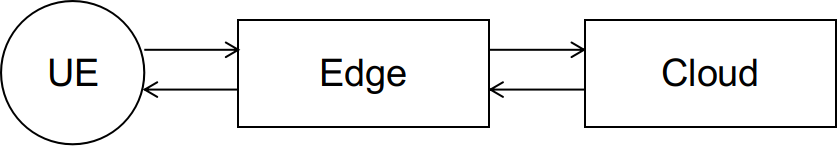
\includegraphics[width=0.8\linewidth]{images/network.png}
        \caption{Network Model for Caching Problem}
        \label{fig:network}
    \end{figure}

    The link between Edge Node and Cloud is called "backhaul link", and the link between Edge node and UE (User Equipment) is called "fronthaul link".
    As we consider the scenario with edge caching, it's reasonable that the delay of fronthaul link is rather fixed only caused by bandwidth restriction. The mobile user (UE) should be allocated with enough communication bandwidth with the support of the initialization procedure, as what we have talked about in the beginning. The backhaul is always assumed with large bandwidth supported by the backbone network, and the propagation and processing delay compose the major factors of the total link-wide delay.

    Furthermore, we denote the the fronthaul delay with a constant $T_0$ as it's rather negligible compared with the backhaul delay. Then we denote the pseudo-backhaul bandwidth with a random variable $BW^{back}$, which could be estimated with large enough on-system data samples in the backbone network.
    
    \subsection{Caching Model}
    As for the caching procedure we described, there are just general files stored encoded in binary format. We consider that files are stored into segments on both Edge and Cloud side, which is easy to quantize the different length of files.The storage capacity of edge cache node is bounded considering energy efficiency and volume limit. But the storage on cloud is assumed to be incredible large.
    
    The files are stored in segments on cloud and each segment is with the same size. The storage is continuous with all the file segments aligned head-to-tail; and for each file, we assume there is one oracle (or called \textit{function}), $\mathcal{D}$ to query the starting and ending index for a certain file.

    However, the transmission time of the fixed-size segments could not be quantized due to the varied transmission delay on backhaul link. The integrity of the received segments is guaranteed by error-correction coding scheme and is not considered in our formulation. And due to the error-correction assumption, the fragment of a segment is meaningless and could not recover the original information without fully received.

    \subsection{Request Problem Definition}
    With the Network and Cache model elaborated above, here we give the description of the whole problem.

    We assume that there are total $N$ files for that user, and the file set is denoted as $\mathcal{F} = \{f_1, f_2, \dots, f_N\}$. Each file is composed of different number of segments, and stored continuously head-to-tail on cloud according to the index as:
    $$
    \mathcal{S_F} = \{S_{1,1}, \dots, S_{1,|f_1|}, \dots, S_{N,1}, \dots, S_{N,|f_n|}\}
    $$
    where $|f_i|$ is the number of segments of $i$-th file, and each segment $S_{i,j}$ is of same size denoted as $l_0$. For convenience of expression, we further define the public query oracle that:
    $$
    \mathcal{D}:f_i \to \{S_{f_i,1}, \dots, S_{f_i,|f_i|}\}, \forall f_i \in \mathcal{F}
    $$
    which is accessible from both Edge and Cloud to obtain the segments set of $i$-th file. The storage capacity of the cache node is denoted as $C$ segments, which is considered rather smaller compared with number of the total file segments.

    The request process $\mathcal{R}(t)$ could be divided into multiple episode, which means that the request could only in initiated after the previous request is been served, as we don't allow batched request in our problem. When one request happens, the cache node should firstly ask the oracle $\mathcal{D}$ to obtain the knowledge of segments set to serve. Then the Edge Node divided the requested segments set into two subset according to the storage: $\mathcal{S}_R^{1}$ for hit segments, $\mathcal{S}_R^{0}$ for missing segments.
    The cache node could serve $\mathcal{S}_R^{1}$ with local hit segments each with fixed delay $T_0$ defined in \ref{net_model}. And the time consumed for $\mathcal{S}_R^{0}$ is what we want to minimize because we notice that the service time is heavily affected from the previous storage state.

    We denote the proactive caching policy set as $\mathcal{A} =\mathcal{F} \times \mathcal{S}$, which implies the complexity of potential action space is non-linear. And then we could formulate stochastic optimization problem as following:
    $$
    \min_{\mathcal{A}} \lim_{T \to \infty} \frac{1}{T} E[\sum_r^{\mathcal{R}(t)} \frac{|\mathcal{S}_{r}^{0}|}{BW^{back}(t)}]
    $$
    which implies that the optimization target is to minimize the average service time for missing segments over all the time. The metric of service time is better than conventional git rate cause the varied delay of backhaul also affects the user experience. And for this stochastic optimization problem, we need powerful algorithm to predict the action with respect to request and delay distribution in real-time.

    In the following chapter, we will formulate this optimization problem as deep reinforcement learning problem, and leverage an existing scheme called A3C to solve the proactive caching problem \cite{a3c}.
\end{section}

\begin{section}{\textsc{AutoCache}: A Proactive Cache Algorithm}
    \label{sec:algorithm}
    In this section, we introduce the algorithm \textsc{AutoCache} to solve this problem. We apply deep reinforcement learning in edge caching, which is able to learn caching policy automatically without any prior programmed control rules or explicit assumptions about the operating environment.
    
    \subsection{Reinforcement Learning Problem}
    Inspired by Pensieve \cite{Pensieve}, we propose an algorithm designed based on reinforcement learning (RL). We firstly rewrite the previous optimization definition in section \ref{sec:formulation} into RL format, then reveal the insights of this problem and develop our algorithm.

    Considering the standard reinforcement learning setting, an agent interacts with environment $\mathcal{E}$ over a number of discrete time steps. At each time step $t$, the agent receives a state $s_t$ and selects an action $a_t$ from some set of possible actions $\mathcal{A}$ according to its policy $\pi$. In return, the agent receives the next state $s_{t+1}$ and receives a scalar reward $r_t$. The return
    $$
    R_t=\sum_{k=0}^{\infty}\gamma^k r_{t+k}
    $$
    is the total accumulated return from time step $t$ with discount factor $\gamma\in(0,1]$. The goal of the agent is to maximize the expected return from each state $s_t$ \cite{rl-intro}.The value of state $s$ under policy $\pi$ is defined as $V^{\pi}(s)=\mathbb{E}[R_t|s_t=s]$ and is the expected return for following policy $\pi$ from state $s$ \cite{DBLP:journals/corr/MnihBMGLHSK16}. The value function can be represented using a neural network, for example, an actor-critic network. The algorithm is proposed to perform online and hoped to achieve high efficiency.

    In our proposed model, the caching agent observes the environment and obtains several signals, including user requests, context information, and network conditions. These signals are assembled into a high-dimensional state input and then fed to the deep neural network embodied convolutional neural networks, which can mine useful information and output the value function or the policy. According to the output, an action is selected, determining the files to be cached at the next slot. The caching agent will receive a reward by observing the caching performance. The aim is to maximize (minimize) the expected accumulated discount reward (cost).

    The system state for this problem is: $\tau$ as last segment downloading time, $B$ as last downloading bandwidth, and $C$ for cache storage expression.

    In order to represent the limits on the storage capacity, the DRL agent makes a decision for each request on whether to store the currently requested file in the cache or not; and if yes, the agent determines which local file will be replaced. For each caching decision, there are $\mathcal{C} \times \mathcal{S} + 1$ possible actions. When $a_i=0$, the currently requested file is not stored, and the current caching space is not changed. When $a_i = n$, where $n\in\{1,2,\cdots,\mathcal{S_F}\}$, the action is to store the currently requested file by replacing the $n$-th file in the cache. The mathematical representation for action over one entry could be formulated as:
    $$
    a_i \triangleq I[C[i]=s], \forall i \in [1, \dots, |C|]
    $$
    where $s \in [0, |\mathcal{S_F}|]$. We define the action space as $\mathcal{A}=\{a_1, a_2, \cdots, a_C\}$. For each file, there are two cache states: cached and not cached. There are also two kinds of actions: find a pair of files and exchange the cache states of the two files; keep the cache states of files unchanged.
    
    We aim to find the optimal caching policy to maximize the expected accumulated discount cost as collection of service time
    $$
    \min E[\sum_{t=0}^{\infty} \gamma^t r_t]
    $$
    , where $\gamma\in(0,1]$ and the reward is defined as
    $$
    r_t = I[\text{in-service}]
    $$
    where the indicator function is noticed by the environment for whether the agent is responding the request in this period. And furthermore, there exists near-optimal heuristic algorithm for the service phase: the cache could stop caching the segments not in $S^{0}_{R}$ but only bypass request for the missing segments from Cloud for this request. This heuristic algorithm could actually be simulated by environment, and not available in formulation of DRL.
    
    \begin{figure}[htp]
        \centering
        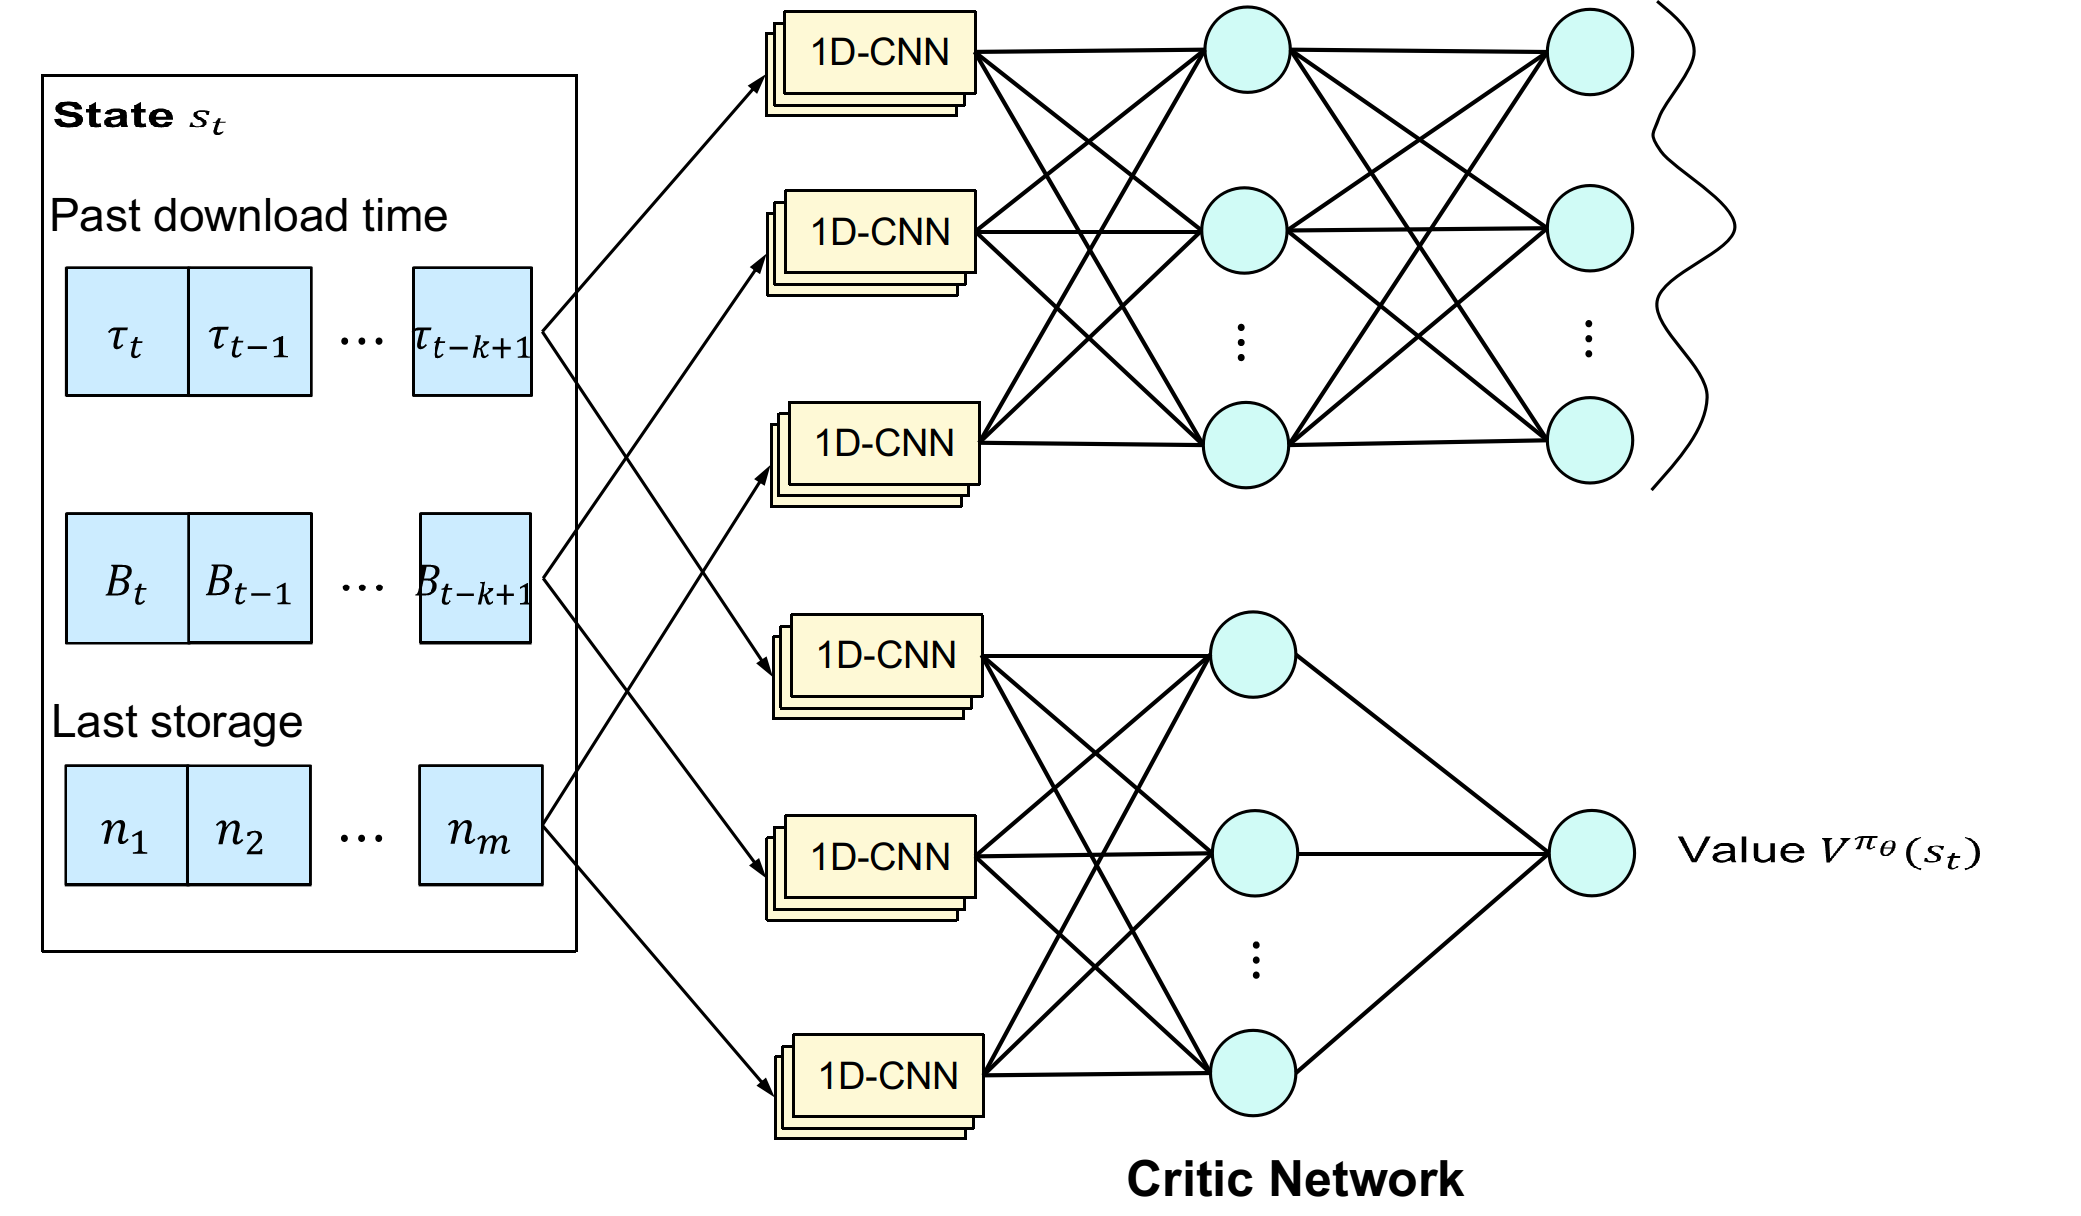
\includegraphics[width=0.8\linewidth]{a3c-network.png}
        \caption{The used actor-Critic algorithm for \textsc{AutoCache}}
        \label{fig:a3c}
    \end{figure}
    
    \subsection{Training Algorithm}
    
    The following training algorithm procedure is abstracted from the original paper \cite{a3c} and take reference from \textit{Pensieve} \cite{Pensieve}.

    Our algorithm firstly obtain the states after taking action.
    Then upon receiving the updated states, the agent needs to generate next action based on the actor's decision: $\pi(s_t, a_t) \to [0,1]^{\mathcal{R}}$. The actor network in Figure \ref{fig:a3c} upper part shows how the action is determined after the states input.
    
    Then it comes to the policy gradient training session. After applying each action, the simulated environment should provide the corresponding cost $r_t$. The actor-critic algorithm the apply a policy gradient method to estimate the gradient of the expected total cost by observing the trajectories of executions obtained by following the policy \cite{Pensieve}. The applied policy gradient is computed as:
    $$
    \nabla_\theta E_{\pi_\theta}[\sum_{t=0}^{\infty} \gamma^ r_t] = E_{\pi_\theta} [\nabla_{\pi_\theta} log_{\pi_\theta}(s,a) A^{\pi_\theta}(s,a)]
    $$
    where $A^{\pi_theta}(s,a)$ is the \textit{advantage} function, which represents the difference in the expected total cost \cite{Pensieve}. The illustration of the approximation is showed in the lower part of Figure \ref{fig:a3c}.

    
    
\end{section}

\begin{section}{Performance Evaluation}
    \label{exp}
    We obtain the real users' data from Google \cite{clusterdata:Reiss2011}, and the actual usage is directly borrowed from cooked data by \cite{Pensieve}. As the data trace following the format as: [timestamp (s), bandwidth (MBps)], we could collect enough data samples under different network conditions, and plot rather accurate CDF (Cumulative Distribution Function) graph versus the value with normalized service time. The experiments details are listed in the following sections. 
    
    \subsection{Simulation Setup}
    We firstly talk about the parameters setup we use and the data trace.
    We implement our algorithm with Tensorflow written in Python. The preliminary for the experiment environment is: Python 3.7+, Tensorflow 1.9+. Our program runs regardless of operating system, but we suggest Linux system for better compatibility. Our experiment following is carried out on Windows Subsystem for Linux (WLS) on Windows 10, and there are 4 parallel agents running on all the 4 CPU cores.

    Then we generate the random user request distribution with the following parameters. 
    The request interval is generated with Poisson Point Distribution with mean as 6 seconds ($\lambda=6$). There are total 6 files on the cloud for the user, and the popularity of files obeys Zipf's law over total files with parameter as $\alpha=1.07$.

    We choose the performance metric only with one cost: average service time. In order to highlight our algorithm performance, we also propose to compare the result from our DRL algorithm with that from heuristic algorithms. We adapt one classical offline algorithm, LRU for comparison. LRU refers to \textit{Least Recently Used}, which discards the least recently used items firstly in cache. The algorithm requires keeping track of the frequency of all the items, and performance passive caching only when the request is initiated.

    The comparison for statistics property of service delay will be discussed in the results section. By taking Google production data trace as evaluation test-bed, we expect our algorithm could outperform the simple heuristic algorithm.    

    \subsection{Results}
    Under the environment and parameters setup in the previous section, we firstly train the A3C neural network for actor and critic with training data. The training process is carried out in a pseudorandom way to enlarge the differences among all of the parallel agents. After enough epoch of training, we test our algorithm with the trained model over test data trace. For fairness, the comparison with LRU is over same data trace set.

    Then we compare \textsc{AutoCache} with classical algorithm LRU. The results for training traces with 1000 samples is shown in Figure \ref{fig:train}; and the results for test traces with 1000 samples is shown in Figure \ref{fig:test}.

    \begin{figure}[htp]
        \centering
        \subfloat[with training data trace]{
            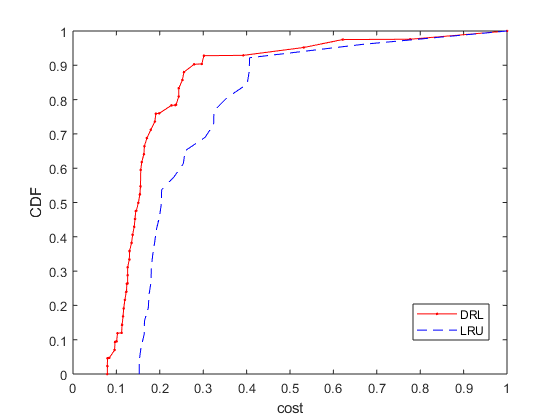
\includegraphics[width=0.45\linewidth]{training.png}
            \label{fig:train}
        }
        \hfill
        \subfloat[with test data trace]{
            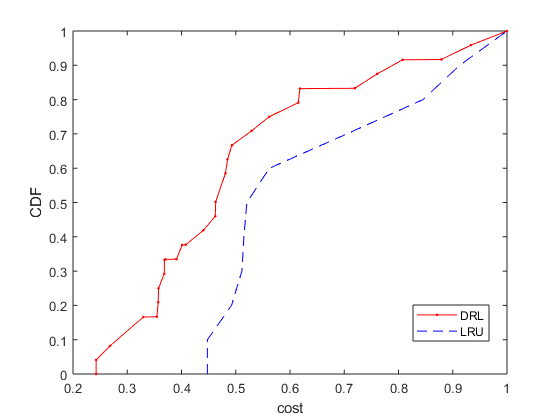
\includegraphics[width=0.45\linewidth]{testing.png}
            \label{fig:test}
        }
        \caption{The CDF of service delay of LRU and DRL algorithm under training and test data trace}
    \end{figure}

    According to the CDF graph, we could find that: whatever in training data trace or not, our algorithm \textsc{AutoCache} could always outperform the classical LRU algorithm as the distribution of service delay is rather prefer to lower side. The drop of average delay would vary from $10\%-15\%$.
\end{section}

\begin{section}{Conclusion}
    \label{summary}
    In this paper, we study one simplified scenario for edge network caching environment. We identify that the single-user-single-cache game could be separated into two phases, proactive caching and passive service, where the transition signal is the user's file request. In the proactive phase, we formulate one reinforcement learning problem and in the second phase we find one heuristic algorithm to efficiently 
    Then we develop our proactive caching prediction algorithm \textsc{AutoCache} with Tensorflow, and compare with classical passive caching algorithm LRU. Over large sample set under different network conditions, the CDF of service time shows that our algorithm could obviously outperform LRU, and the storage varies slowly with less bandwidth consumed.
\end{section}

% \section*{References}
\bibliographystyle{IEEEtran}
\bibliography{main.bib}

\end{document}